% 薄透镜

% 球形界面
% 未完成: 改名为透镜

\pentry{折射定律\upref{Snel}}

\subsection{单个球面的成像公式}
\begin{figure}[ht]
\centering
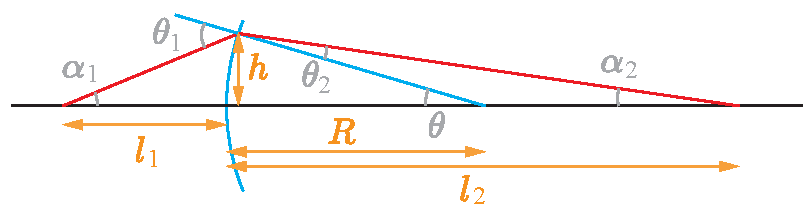
\includegraphics[width=12.5cm]{./figures/ThnLen1.pdf}
\caption{单球面成像} \label{ThnLen_fig1}
\end{figure}

如\autoref{ThnLen_fig1}, 我们考虑两种折射率分别为 $n_1$ 和 $n_2$ 得介质被一个球面划分为左右两部分. 当光线从左边入射时, 经过界面反射.

\textbf{傍轴条件}: 图中所有角度都很小\footnote{即 $\sin\beta \approx \tan\beta \approx \beta$, 见 “小角正弦极限\upref{LimArc}”}. 球面近似是平面, 球面上任意一点横坐标相同.
\begin{equation}
l_1 \alpha_1 = l_2 \alpha_2 = R\theta
\end{equation}
由三角形性质得
\begin{equation}
\alpha_1 = \theta_1 - \theta \qquad
\alpha_2 = \theta - \theta_2
\end{equation}

\begin{equation}
n_1 \theta_1 = n_2 \theta_2
\end{equation}
消去 $\theta_1$ 和 $\theta_2$ 得
\begin{equation}
\frac{n_1}{l_1} + \frac{n_2}{l_2} = \frac{n_2 - n_1}{R}
\end{equation}
这已经比较接近凸透镜成像公式了. 注意当 $l_1$ 或者 $l_2$ 取负数时同样成立, 这意味着物或者像在透镜的另一侧(即虚物或者虚像). 若透镜的圆心在左侧, 将式中 $R$ 也改为负数即可(请读者自行证明这两个结论). 最后注意我们并不要求式中 $n_1, n_2$ 哪个更大.

\subsection{薄透镜}
%图未完成

如果一个透镜的两个面可以近似为球面, 且它们之间的距离比起物距和像距来可以忽略不记, 那么我们就称它为\textbf{薄透镜}. 我们假设透镜外介质的折射率为 $n_1$, 透镜内折射率为 $n_2$. 我们另透镜一侧的半径为 $R_1$, 物距为 $u$, 像距为 $v_1$, 另一侧半径为 $R_2$(另焦点在另一边为正), 物距为 $u_2$, 像距为 $v$. 于是有
\begin{equation}\label{ThnLen_eq1}
\frac{n_1}{u} + \frac{n_2}{v_1} = \frac{n_2 - n_1}{R_1}
\end{equation}
\begin{equation}\label{ThnLen_eq2}
\frac{n_2}{u_2} + \frac{n_1}{v} = \frac{n_2 - n_1}{R_2}
\end{equation}
由于透镜厚度可以忽略, 任何情况下都有
\begin{equation}\label{ThnLen_eq3}
v_1 = -u_2
\end{equation}
将\autoref{ThnLen_eq1} 与\autoref{ThnLen_eq2} 相加再用\autoref{ThnLen_eq3} 消去含有 $v_1$ 和 $u_2$ 的两项, 就得到了熟悉的\textbf{薄透镜成像公式}
\begin{equation}
\frac{1}{u} + \frac{1}{v} = \frac{1}{f}
\end{equation}
其中
\begin{equation}
\frac{1}{f} = \qty(\frac{n_2}{n_1} - 1) \qty(\frac{1}{R_1} + \frac{1}{R_2})
\end{equation}
再次声明这里使用的正负号规范: 实物距离为正, 实像距离为正, 凸透镜半径为正; 反之为负.

% 例题未完成.

\subsection{薄透镜叠加}
与上一节同理, 若两个焦距分别为 $f_1$ 和 $f_2$ 的薄透镜叠加, 当其间距远小于物距和像距时, 合成后的透镜焦距 $f$ 满足
\begin{equation}\label{ThnLen_eq4}
\frac{1}{f} = \frac{1}{f_1} + \frac{1}{f_2}
\end{equation}

推导: 另第一个透镜的物距为 $u$, 像距为 $v_1$, 第二个透镜物距为 $u_2$, 像距为 $v$, 由于两透镜距离可忽略, 第一个透镜的实像像距等于第二个透镜的虚物物距, 所以分别可以列出
\begin{equation}
\frac{1}{u} + \frac{1}{v_1} = \frac{1}{f_1}
\end{equation}
\begin{equation}
\frac{1}{u_2} + \frac{1}{v} = \frac{1}{f_2}
\end{equation}
\begin{equation}
v_1 = -u_2
\end{equation}
联立得
\begin{equation}
\frac{1}{u} + \frac{1}{v} = \frac{1}{f_1} + \frac{1}{f_2}
\end{equation}
令组合透镜的等效焦距为 $f$, 即等式右边为 $1/f$, 得到\autoref{ThnLen_eq4}.
